\documentclass[11pt,a4paper]{article}
\usepackage[utf8]{inputenc}
\usepackage{amsmath}
\usepackage{amsfonts}
\usepackage{amssymb}
\usepackage[spanish]{babel}
\usepackage[usenames,dvipsnames,svgnames,table]{xcolor}
\usepackage{graphicx}
\usepackage{subfigure}
\usepackage{setspace}
\usepackage{enumerate}
\usepackage{ragged2e}
\usepackage[margin=10pt,font=small,labelfont=bf,labelsep=endash]{caption}
%\usepackage{hyperref}
\usepackage[bookmarks = true, colorlinks=true, linkcolor = black, citecolor = black, menucolor = black, urlcolor = black]{hyperref}
\usepackage{indentfirst}
\usepackage{pdfpages}
\usepackage[left=2cm,right=2cm,top=2cm,bottom=2cm]{geometry}
\usepackage{fancyhdr}
\usepackage{listings}
\usepackage{tabularx}
\usepackage{color}
%\usepackage[maxbibnames=99,sorting=none,backend=bibtex]{biblatex}
%\addbibresource{Ref.bib}
\usepackage{colortbl} 
\usepackage{array}
\usepackage{upgreek}
\usepackage{matlab-prettifier}

\title{Plan de Negocios 2021}
\author{Pablo Ezequiel Córdoba - Federico Cravero - Paul Andrés Coronado Romero}
\date{June 2021}

\begin{document}

\maketitle
La carátula se la come, usamos la que tengo una vez terminado esto.

Tomatelá de acá te dije

Me importa un carajo
\pagebreak

\tableofcontents

\section{Resumen Ejecutivo}

\textbf{Acá iría un chamuyo para engatusar a los inversores, eso quizás es más conveniente hacerlo al final, por si hay algún cambio en el proyecto.}

\section{Análisis Estratégico y Competitivo}
% * <Federico Cravero> 12:51:14 11 Jun 2021 UTC-0300:
% estrategia diferencial
% * <Paul Romero> 11:41:14 10 Jun 2021 UTC-0300:
% Me parece que es muy importante y que no debe faltar poner dentro de las subsecciones que nuestro negocio/mciroemprendimiento se va a encontrar dentro de San Luis Capital y cúal es el mercado al que nos estamos adentrando (como lo hizo Kevin)

\subsection{Descripción del mercado actual}

A raíz de la pandemia del Coronavirus, estudios han revelado un aumento importante en la demanda de las computadoras, tanto portátiles como de escritorio, siendo este un mercado muy demandante para los tiempos actuales, en donde se ha incrementado el trabajo y el estudio desde casa.

En Argentina, hay varias páginas web y locales correspondientes al mercado de venta de insumos y servicios informáticos, los cuales, los más importantes se encuentran en la provincia de Buenos Aires.

Particularmente, en la ciudad de San Luis, no hay demasiados comercios que se dediquen a dicho mercado. O no poseen la movilidad necesaria para asistir a la vivienda del cliente y satisfacer su demanda. Ya que además, por lo general, no cuentan con una página web, en donde se pueda realizar una compra online y retirar en el local, o simplemente que el cliente reciba su producto desde la comodidad de su casa. Como así también, vender o prestar servicio a una reparación de equipos antigüos. 

Además, es un hecho que tanto los clientes que saben más sobre componentes de Pc como aquellos que no prefieren comprar online debido a la diferencia de precios sobre un mismo producto entre los aquellos ofrecidos por un microemprendimiento fuera de la provincia y de la provincia. 

Por lo tanto, se propone dos cosas:
\begin{itemize}
    \item Un negocio de venta de insumos informáticos, específicamente componentes de PC (todo lo necesario para armar una computadora desde cero con los requisitos del cliente). También proporcionar un servicio técnico de computadoras adaptado a las nuevas tecnologías, para la provincia de San Luis.
% * <Federico Cravero> 19:49:01 02 Jun 2021 UTC-0300:
% $todo lo necesario para armar una computadora desde cero con los requisitos del cliente$
    \item Y, lo más importante, ofrecer la seguridad a los clientes de que los productos sean de buena calidad y que el servicio técnico es el óptimo para que estos nos vuelvan a elegir. De esta forma, se busca diferenciarnos de la competencia. 
\end{itemize}


\subsection{Participación de mercado para marcas representativas}

Para el mercado de venta de componentes de PC, las marcas más representativas que se pueden encontrar son \textit{AMD}, \textit{Intel} para procesadores, \textit{NVidia} y \textit{AMD Radeon} para placas gráficas, como así también \textit{MSI}, \textit{Asrock}, \textit{Gigabyte} y \textit{ASUS} para placas base. Finalmente para almacenamiento \textit{Redragon}, \textit{Kingston} y \textit{Western Digital} entre otros. 

\subsection{Análisis FODA} 
\subsubsection{Fortalezas} 
\begin{itemize}
    \item Se brindará un servicio completo, de venta de insumos y servicios informáticos, el cual no se realiza de forma adecuada en la zona zona.
% * <Federico Cravero> 17:45:09 09 Jun 2021 UTC-0300:
% Tenemos que ver la venta web
    \item Se brindará un servicio de venta web, que permitirá distintas formas de pagos. La plataforma permitirá que los empleados asesoren a los clientes que lo precisen.
    \item Buen manejo de las redes sociales para dar a conocer y publicitar el microemprendimiento.
    \item Se brindará un servicio de delivery para aquellos clientes que no puedan trasladar su equipo al local.
\end{itemize}

\subsubsection{Debilidades} 
\begin{itemize}
    \item Nuevos en el mercado.
    \item Falta de experencia práctica en el mundo de los negocios.
% * <Paul Romero> 17:52:37 09 Jun 2021 UTC-0300:
% Calidez de microemprendimiento, algo así
% ^ <Federico Cravero> 11:24:16 11 Jun 2021 UTC-0300:
% Para mi va de la mano con la antigüedad
    \item Carencia de clientes recurrentes.
    \item Falta de trayectoria.
\end{itemize}

\subsubsection{Oportunidades}
\begin{itemize}
    \item Alto crecicimiento que se puede tener en este sector.
    \item Mercado carente de monopolio y oligopolio.
    \item Aumento de la demanda debido a la pandemia.
\end{itemize}

\subsubsection{Amenazas}
\begin{itemize}
    \item Posibilidad de entrada de competidores con un servicio similar.   
    \item Escasez de placas de video. Tanto AMD como NVIDIA han confirmado que el stock de placas de video seguirá siendo prácticamente nulo durante todo el primer trimestre de 2021. Esto significa que no veremos síntomas de mejora hasta el segundo trimestre de 2021. Dando como resultado un aumento entre un 80\% y 200\% de estos productos.
    \item Precios de los componentes sujeto al cambio volátil del dolar.
    \item Parte de los posibles clientes prefieren la compra a negocios fuera de la provincia.
    \item Dificil adquisición de productos por parte de los proveedores debido a la pandemia.
    \item Inminente digitalización de las ventas debido a la pandemia.
    
\end{itemize}
% * <Pablo Ezequiel Córdoba> 18:07:39 09 Jun 2021 UTC-0300:
% Como has estado completando la info?
% Te basaste en los informes que pasó alan y partiste de ahí investigando?
% Pulpo marak
% Si, y mirando el video de plan de negocios que está separado digamos lo que serían las secciones 

\subsection{Evaluación de la necesidad de nuevos productos}
La industria del hardware es una de las que nunca dejan de avanzar, por lo que cada año salen nuevos productos que ofrecen mejores prestaciones lo que trae como consecuencia la rápida obsolecencia de aquellos con mayor tiempo en el mercado. Por lo tanto, como negocio, se debe de tratar de ofrecer los últimos productos en componentes de Pc para poder satisfacer la demanda de posibles clientes.

Si solo se ofrece productos lanzados hace más de dos años, está la posibilidad de que el posible cliente pierda el interés en este negocio.

\subsection{Atributos del producto y servicio}
Al ser la reventa de insumos informáticos la activiadad que impulsa este microemprendimiento, se ofrecerán productos originales, actualizados, de la mejor calidad y a precios realistas.

% * <Paul Romero> 13:42:29 11 Jun 2021 UTC-0300:
% Los atributos son las características que tiene ya sea un producto o un servicio en relación a su comercialización, es decir, son todos aquellos aspectos que lo hacen partiendo desde la idea, a la fabricación y finalmente la imagen del producto (etiquetas, envase, color, sabor, olor y más dependiendo del tipo que sea) o sea que los atributos son aquellos que en conjunto determinarán el éxito del producto.
Los atributos de este servicio son:
\begin{itemize}
    \item Brindar un buen asesoramiento.%como ingenieros que somos
    \item Brindar la mejor atención al cliente.
    \item Garantizar un servicio técnico óptimo.
    \item Brindar los medios de pagos más usados
    \item Consultas online mediante chat o llamada telefónica.
    \item Armar combos de componentes y ofrecer ofertas para estos.
    %\item %ACA QUIERO PONER ALGO QUE LE DEMOS NOSOTROS AL CLIENTE PARA QUE NOS SIGA COMPRANDO (ponele, mientras más compras le damos ofertas así a lo mercadolibre). Si a ustedes se les ocurre algo ponganlo acá pls los tkm gatos
    \item Brindar un servicio de delivery eficiente y confiable para el transporte de equipos de los clientes.
\end{itemize}


%Los atributos del producto serán:
%\begin{itemize}
%
 %   \item Atributos físicos: Datos precisos sobre las dimensiones, peso, características, compatibilidad, disponibilidad y precio del mismo.
%    \item Se ofrecerá una amplia variedad del mismo con la mejor calidad y precio
%\end{itemize}




\subsection{Análisis de las barreras de ingreso y egreso}

%cierre de fronteras por covid

\subsection{Hipótesis de posicionamiento}

%posicionamiento: frente a tu cola


\section{Análisis e investigación de mercado}

El mercado que preside en San Luis, no es amplio, ni tampoco posee locales que se puedan llamar centrales o importantes, lo que más se destaca es que todos o la gran mayoría se ubican por la zona céntrica de la ciudad, por lo tanto, para poder triunfar, se debe buscar un lugar bastante grande, considerando a los clientes que pueden llegar a asistir, y además en lo posible con un estacionamiento.

El presupuesto inicial debe ser considerable, debido a los altos costos de los componentes, ya que los mismos varían con la devaluación de la moneda argentina, e inclusive impuestos por compras al exterior (del país) de aproximadamente un $64\%$. Además el presupuesto va a depender de los socios Cravero, Romero y Córdoba. 

Como el presupuesto depende de los socios y este fue destinado para otros aspectos, se extraen los siguientes datos públicos: Según el Instituto Nacional de Estadística y Censos (\textbf{I.N.D.E.C}), en el último trimestre del año pasado (2020) las ventas de productos electrónicos incrementaron en un $66,8\%$ respecto al mismo período en 2019 a raíz de la pandemia del Coronavirus, además se registró que en Argentina, el $63,8\%$ de los hogares urbanos tiene acceso a computadora y el $90\%$, a internet. La fuerte demanda impulsada por el trabajo desde el hogar y las necesidades de aprendizaje electrónico ha superado las expectativas anteriores y una vez más ha puesto a la PC en el centro de la cartera de tecnología de los consumidores.

Así mismo, la ciudad de San Luis tiene una población de 202300 habitantes (2015) y se estima que aproximadamente hay 221734 para el año 2021. Como a partir de los 4 años los niños pueden utilizar una computadora, y obviamente será costeado por los padres, hay un gran porcentaje de clientes potenciales, ya sea para comprar algún componente o simplemente para reparar el equipo.

\section{Estudio de la competencia}
Para realizar un análisis de la competencia, se considera únicamente a aquellos negocios en San Luis que ofrecen lo mismo que nuestra empresa. Es decir, servicio técnico de computadoras y venta de insumos de informática. 

En este rubro, los locales que realizan una actividad similar dentro de la provincia son: \textit{Compumundo, Pablo Computación, Tu PC, Compusystems}, ya que hay muchos otros que desempeñan únicamente una de las tareas y no ambas.

Una vez que se identifican las competencias, se procede a realizar una tabla de ponderación de 1 a 5 (menos significante a más significante) entre los competidores y \textbf{NOMBRE DEL EMPRENDIMIENTO}, donde se tienen en cuenta algunos factores críticos para el éxito del negocio.
% * <Federico Cravero> 11:22:44 11 Jun 2021 UTC-0300:
% Nombre del emprendimiento

%\begin{figure}[h]
%     \centering
%     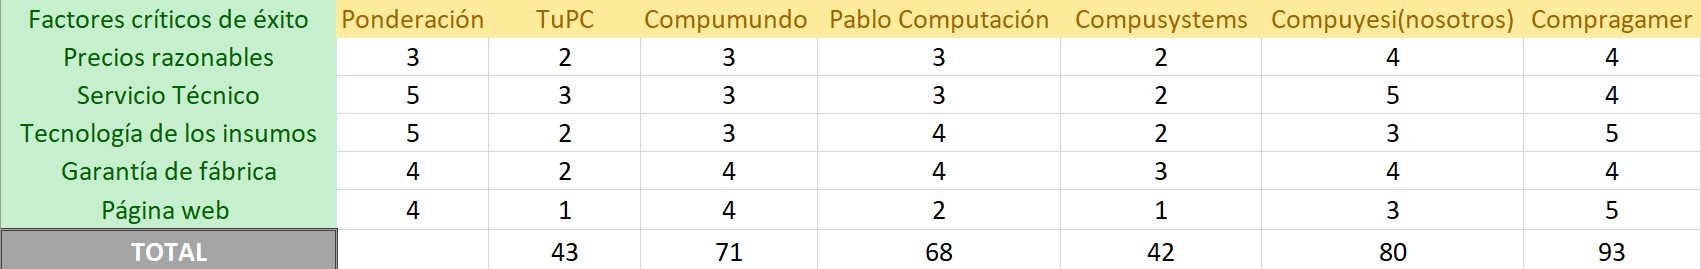
\includegraphics[width=12cm]{Tabla_ponderacion.png}
%     \caption{Tabla de ponderación para determinar el competidor directo.}
%     \label{fig:Tabla_ponderación}
%\end{figure}

	%\	\begin{figure}[h]
	%	\centering
	%	\captionsetup{justification=centering}
	%	\includegraphics[width=0.2\textwidth]{face_segments}
	%	\caption{Сегменты лица, обрабатываемые независимо: глаза, нос, рот, окружающая область. \cite{quality_measure}}
	%	\label{fig:face_segments}
	%\end{figure}

Como se muestra en la FFFFFF, se encuentra que para la ponderación realizada, el competidor directo es \textit{Compumundo}.

\textbf{Tabla de ponderación}

% * <Paul Romero> 17:53:33 09 Jun 2021 UTC-0300:
% Competencias directas: Pablo computación, [insertar más nombres por favor wey no mames]

% * <Pablo Ezequiel Córdoba> 09:25:08 11 Jun 2021 UTC-0300:
% competencias directas sale con el excel, vete a chingar a otra parte :P
\section{Segmentación} 

Se busca que el negocio ofrezca productos de componentes de computadoras. Es decir: fuente de alimentación, microprocesadores, placas madres, placas de video, memoria de almacenamiento, memoria RAM, coolers, pasta térmica, gabinetes. Así también como periféricos: mouse, teclado, monitor,auriculares,micrófonos, joysticks. E insumos de informática: cables USB, antenas wifi, cables HDMI, etc.
% * <Paul Romero> 12:38:44 11 Jun 2021 UTC-0300:
% No sé si ponerlo acá o en "atributos de producto y servicio"

El mismo está orientado para clientes que posean un alto y/o un medio nivel adquisitivo (independientemente de su conocimiento técnico sobre componentes de pc), debido a que los componentes más recientes o más nuevos son más caros, mientras que aquellos productos que llevan un tiempo en el mercado, son más accesibles, dependiendo de la tecnología con que se han fabricado.


Las temporadas altas para la venta y el servicio técnico son las mismas. Estas ocurren en las vacaciones de invierno y verano y el inicio de clases. Es decir, los meses de  enero,febrero, marzo, julio y diciembre.
% * <Federico Cravero> 11:45:13 13 Jun 2021 UTC-0300:
% Agregar semanas de descuento como black friday

Además, la frecuencia de compra []
% * <Paul Romero> 13:12:37 11 Jun 2021 UTC-0300:
% NO ENTENDI SI LA FRECUENCIA DE COMPRA ES CON RESPECTO A CADA CUANTO SE VENDE EL PRODUCTO
% O A CADA CUANTO UN MISMO CLIENTE COMPRA EL PRODUCTO


\section{Posicionamiento}
% * <Federico Cravero> 18:10:37 09 Jun 2021 UTC-0300:
% Faltan secciones, agregar las que falten agregame esta

\section{Mercados Potencial y Mercado Meta}

%criterio y metodologia
%encuestas públicas

\section{Plan de Marketing}

La propuesta comercial única que ofrece el micoremprendimiento es brindar información confiable y certera, un servicio de venta y post-venta impecable para que nuestros clientes siempre vuelvan a elegirnos.

El proyecto busca aquellas personas mayores de 18 años con una idea de lo que necesitan y que, con ayuda del acesoramiento profesional del personal se decidan por los productos de calidad que ofrecerá el mismo. 


%Analisis de la situacion actal
%FODA
% * <Federico Cravero> 10:29:16 13 Jun 2021 UTC-0300:
% -La venta y consulta vía web será atendida inmediatamente en horas de trabajo, más aún en tiempos de pandemia
% -Los clientes serán atendidos solo por personal capacitado 
% -El servicio de delivery quiere llegar a los clientes que no poseen el medio para llevar sus equipos de trabajo a nosotros

%-cliente ideal 
% * <Federico Cravero> 12:11:13 12 Jun 2021 UTC-0300:
% Aquellas personas mayores de 18 años con una idea definida en mente de lo que necesitan y que por medio de nuestro asesoramiento profesional se decidan por nuestros productos de calidad. Aquellos que debido a la pandemia necesitan un equipo nuevo o renovarlo.

%propuesta comercial unica
% * <Federico Cravero> 12:08:52 12 Jun 2021 UTC-0300:
% Brindar información confiable y certera, un servicio impecable y el mejor servicio de post-venta para que nuestros clientes siempre vuelvan a elegirnos.

%Analisis de la competencia
%presupuesto y volumen de negocio q manejan
% * <Federico Cravero> 12:16:16 12 Jun 2021 UTC-0300:
% El volumen de negocio de la competencia.... no tengo idea

%precios de sus productos y servicios
% * <Federico Cravero> 12:15:31 12 Jun 2021 UTC-0300:
% Los precios de la competencia local suelen estar muy inflados por lo que los potenciales clientes prefieren comprar fuera de la provincia

%proceso de ventas
% * <Federico Cravero> 12:13:55 12 Jun 2021 UTC-0300:
% En su mayoría no realizan mucha publicidad debido al reducido numero de locales de este rubro

%como consigue clientes

%Objetivos
% * <Federico Cravero> 12:29:31 12 Jun 2021 UTC-0300:
% -Conseguir un buen posicionamiento en el mercado local en el primer año
% -Tener la preferencia de nuestros clientes (de insumos) como su servicio técnico de confianza
% -Puto el que lee
% -


%4P

\section{Recursos Humanos}

%habría que hacer un organigrama con los distintos sectores en el microemprendimiento, si se terceriza alguna actividad, si se contrata personal (no dice mucho mas el profe)
Para que el negocio prospere, es necesario que los socios Cravero, Romero Coronado y Córdoba estén presentes en varias de las actividades que se deben realizar, terceriazando lo menos posible, para así llevar a cabo una expansión en algún futuro y por supuesto lograr rentabilidad.

En la FFFFFFFF se muestra el organigrama que se va a empeñar para la realización de la actividad propuesta. En donde, se puede observar que los únicos sectores tercerizados son para la \textbf{contaduría} y para el \textbf{desarrollo y mantenimiento web} de la página del negocio. Por más que los socios se encuentren en distintas tareas, las mismas se van a ir organizando dinámicamente para evitar retrasos, por ejemplo, si hay muchos clientes en un determinado momento o día, entre los socios se determinará si es necesario que los tres estén presentes, pausando temporalmente el trabajo que estén realizando en ese momento.

% * <Pablo Ezequiel Córdoba> 13:19:23 13 Jun 2021 UTC-0300:
% Imagen del organigrama
%\begin{figure}[h!]
%    \centering
%    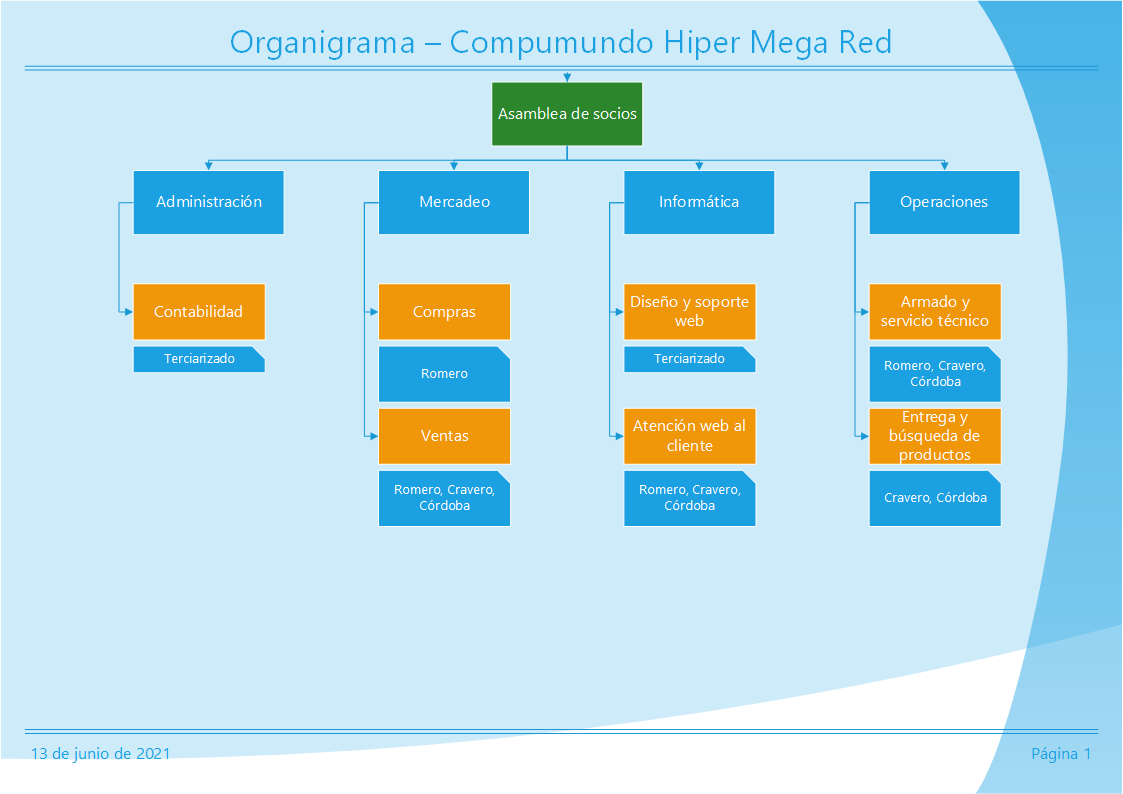
\includegraphics[width=16cm]{Organigrama.png}
%    \caption{Organigrama de Compumundo Hiper Mega Red}
%    \label{fig: Organigrama}
%\end{figure}


\section{Recursos e inversiones}

% * <Paul Romero> 10:51:37 13 Jun 2021 UTC-0300:
% De esto me encargo yo lindo -Pulpo
% Qué tenemos? Qué necesitamos?

Los recursos que el negocio necesita son:
\begin{enumerate}
    \item Local: Se necesita un domicilio legal y real para el negocio. Se decidió alquilar el local comercial 4 Torre República del Líbano ubicado en República del Libano entre las calles Lamadrid y San Juan, el cual tiene un espacio de de 40 $mt^2$. A continuación se muestra el plano del local, su ubicación en Google maps y uan vista de frente de este.
    %    \begin{figure}[h!]
		%	\centering
		%	\subfigure[ Ubicación Google Maps.]{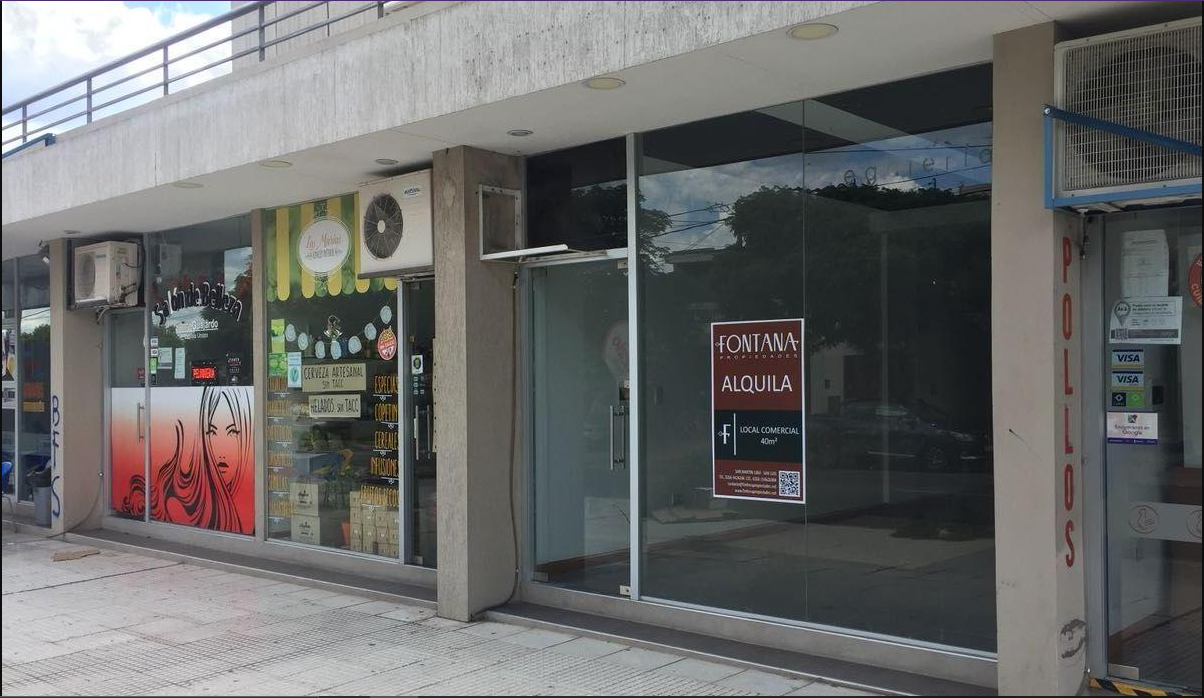
\includegraphics[width=60mm]{local_frente.png}}
		%	\subfigure[Foto de frente]{
\includegraphics[width=60mm]{local_gmaps.png}}
		%	\subfigure[Plano]{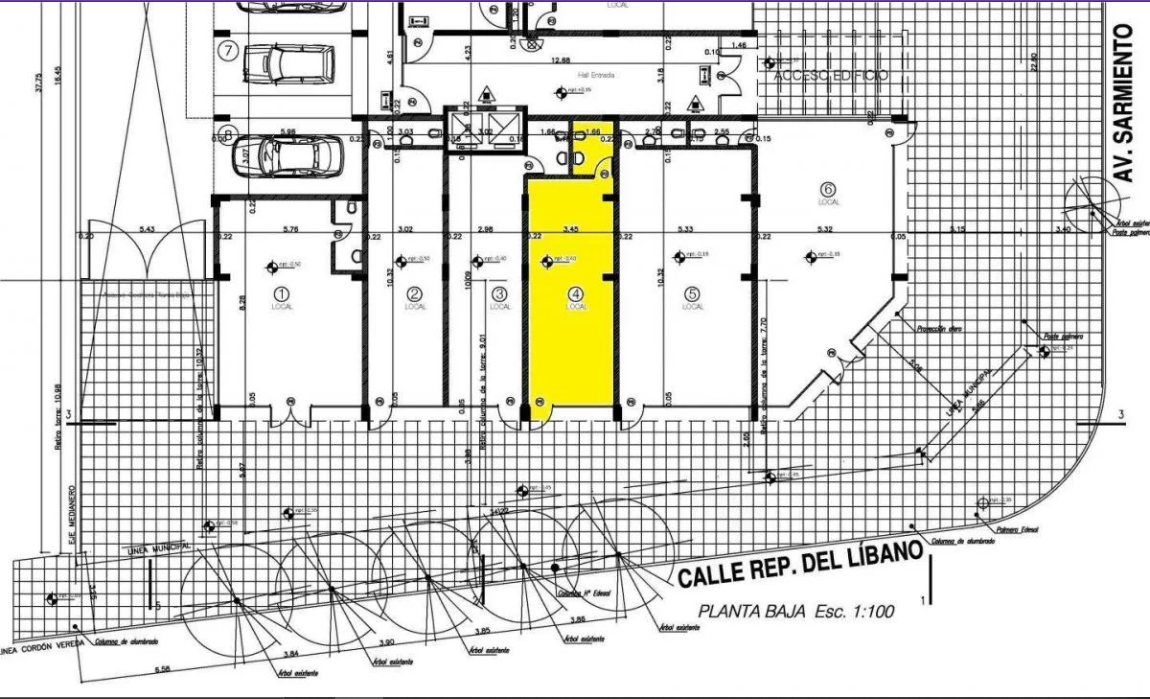
\includegraphics[width=120mm]{local_plano.png}}
		%	\caption{Local que busca utilizar el negocio.}
		%	\label{fig:local}
	%	\end{figure}
	Su costo es de \$17.500,00 más \$2.500,00 por expensas al mes.
    \item Página Web: Al igual que se necesita un lugar físico, también se necesita de un lugar en el internet debido a los tiempos que corren. Sobre esto se encargará un tercero para el diseño de la pagina.
    
        El costo para el dominio de la página web (\textit{.com.ar}) es de \%270.00 al mes.
    \item Página en Instagram: Esta página será utilizada para publicitar el negocio, informar sobre precios, ofertas, etc. Su costo es gratuito, solo se necesita de alguien que se encargue de manejar la página, el cual puede ser cualquiera de los 3 gerentes.
    \item Vehículo: Para el transporte de los productos, es necesario contar con un vehículo utilitario. Por lo tanto se decidió en adquirir un Fiat Fiorino 2021 GNC/Nafta.
        %\begin{figure}[h]
    %     \centering
    %     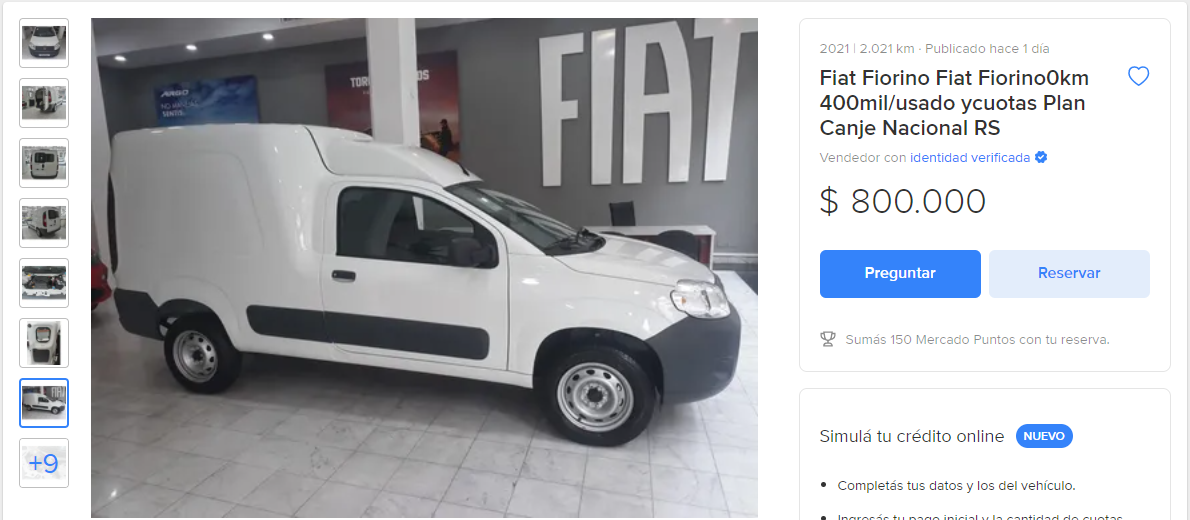
\includegraphics[width=12cm]{auto_ML.png}
    %     \caption{Publicación de venta.Fiat Fiorino 2021.}
    %     \label{fig:Auto}
    %\end{figure}
    El cual posee un coste de \$800.000,00.
    \item Insumos: Los bienes que se comprarán al por mayor y se venderán en el negocio. Esto se profundiza más en la planilla de cálculos. Su costo total es de []
    \item Preparación de local: Comprar vitrinas, estantes, etc 
\end{enumerate}

Los recursos que el negocio ya posee son todas las herramientas necesarias para el servicio técnico.

Por lo tanto, teniendo en cuenta todo lo expresado, se muestra a continuación una tabla con el valor del monto inicial necesario para comenzar con el negocio durante el primer año.



\section{Factibilidad Técnica}
\section{Factibilidad Económica}
\section{Factibilidad Financiera}
\section{Análisis de sensibilidad}
\section{Conclusiones}
\section{Anexos}
\subsection{Bibliografía}
%https://www.infobae.com/america/agencias/2020/07/09/ventas-de-pc-aumentan-ante-recuperacion-de-suministro-y-demanda/
%https://www.indec.gob.ar/indec/web/Nivel3-Tema-4-26
%https://www.muycomputer.com/2021/01/14/escasez-tarjetas-graficas-consejos/
%https://www.zonaprop.com.ar/propiedades/local.-republica-del-libano-43056032.html
%https://auto.mercadolibre.com.ar/MLA-925142209-fiat-fiorino-0km-500milusado-ycuotas-plan-canje-nacionalrs-_JM#position=1&search_layout=grid&type=item&tracking_id=5ec8a294-5c4f-47a6-a612-c2adde8b1028
\end{document}


